%
\section{Evaluation and Discussion}
\label{sec_eval}
\label{sec_conclusion}

\subsection{Benchmarks}
To evaluate our tool, we created a benchmark set containing several images where we manually marked the insects.
The result of one benchmark run is expressed as \textit{Recall}, \textit{Precision}, and \textit{F-Measure} \cite{f_measure}.
Although F-Measure is a very common way to measure the quality of results, we consider changing  to another method that puts a higher weight on the quantity of results. 
Usually, it would be easier to refine existing results than to find additional insects. 
Also, when looking for false positives, it is possible that true positives are found because the bounding box did not fit correctly.
However, it is more useful to see an image of multiple insects or a cropped insect instead of no result at all.

The test set is crucial for the accuracy of the benchmark. 
It is always good to have a large test set to improve the accuracy of the benchmark.
Therefore continuous extending of the test set is needed. 

\subsection{Results}

Running the benchmark on our test set yields the following results:
%
\begin{description}
	\item[Recall] 0.82
	\item[Precision] 0.80
	\item[F-Measure] 0.81
\end{description}
%
The used method consists of the automated template extraction by contour detection, followed by a template matching with the extracted template.

In our test set we have images of well-shaped insects, like butterflies, and different bugs,
but also images of border cases, like insects with transparent wings, stick insects, or insects which are missing some parts of their body.
Those border cases cause a worsening of our benchmark results.
Using a slightly smaller test set, where we only use the common cases, we can achieve much better results:
%
\begin{description}
	\item[Recall] 0.90
	\item[Precision] 0.97
	\item[F-Measure] 0.94
\end{description}
%
\subsection{Discussion}
When executing the benchmark, there is an option to enable a mode to see the evaluated image.
By showing all false and true positives and true negatives it is possible to see what causes the resulting numbers.
The main problem for not having 100\% lies in the diversity of the insects:
Butterflies of the same class often have differing patterns on their wings.
Also differences in color and size are serious, especially between male and female ones of the same species.
Another problem is the condition of the insects:
Some animals have missing parts like wings or legs or they differ in the folding of their wings.
Furthermore sometimes the insects are aligned horizontally and sometimes vertically in one box, so that the template won't find all insects of one alignment.
The first box in Figure \ref{fig:diverse} shows such a high diversity like missing wings.

The condition of the box where the insects are in is another influence on the result.
Sometimes the background of the images has dirt on it, that makes it hard to find a difference to the insects, especially if they have transparent parts like in the second box of Figure \ref{fig:diverse}

\begin{center}
	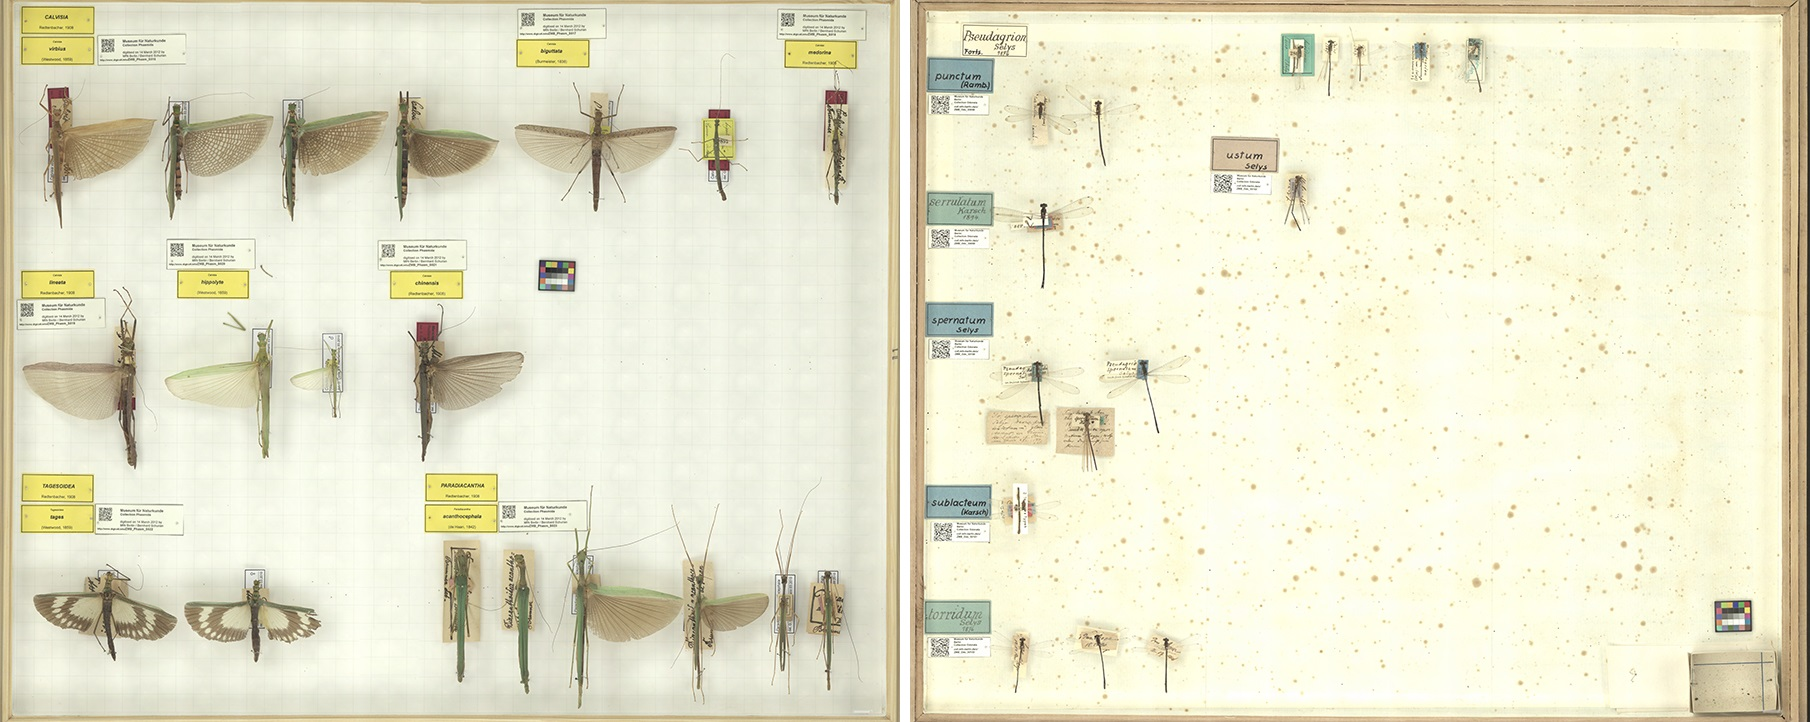
\includegraphics[width=1\textwidth]{images/diversity_dirt.jpg}
	\captionof{figure}{High diversity in one box and dirt in the other one}
	\label{fig:diverse}
\end{center}
All these points make it hard to have a result close to 100\%.
But an F-measure of 94\% is still a very good result and even 81\% with a lot of edge cases is pretty good.

\subsection{Machine Learning}
As described in Section \ref{sec_concepts}, using an SVM is a Machine Learning approach on classification of images.
In the process of developing our tool, we also implemented a SVM, to see if it fits our purposes.
We did not use it in our final method, since a really big training data set is required, which we did not have at that time.
But given proper training data, an SVM would be a valid classification method.

\subsection{Future Work}
Since we can get the classification of the specimen in a picture out of the QR-code, it should be possible to improve the template extraction.
If there is an online-service for getting images of insects by their name, the result of the automated template extraction could be verified on a much more precise level.

Another idea is to have a feedback for the user to show him critical findings or pictures with no matches at all.
Furthermore before processing all images, the software could just generate all templates and show suspect ones to the user to verify if it is a good template or just a label or QR-Code.

In a separate preprocessing step it can be useful to remove all labels and QR-codes from the image before looking for a template.
We spend a lot of time at this, but found no satisfying results without deleting true positives.

As mentioned before, with the help of a large trainings set, Machine Learning could be an interesting method to verify findings or to improve the segmentation.
Such training sets could be gathered from other sources, where an annotation already has been done.
